\documentclass[tikz, border=10pt]{standalone}
\usepackage{tikz}
% Añade aquí cualquier librería que uses, ej: \usetikzlibrary{3d}

\begin{document}
    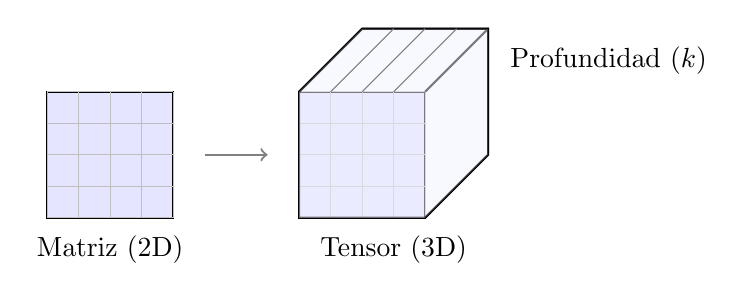
\begin{tikzpicture}[scale=0.8]
        % Matriz (2D)
        \begin{scope}[shift={(0,0)}]
            \draw[thick, fill=blue!10] (0,0) rectangle (2,2);
            \node at (1, -0.5) {Matriz (2D)};
            \draw[step=0.5, gray!50, thin] (0,0) grid (2,2);
        \end{scope}
        
        % Flecha
        \draw[->, thick, gray] (2.5, 1) -- (3.5, 1);
        
        % Tensor (3D)
        \begin{scope}[shift={(4,0)}]
            % Cara frontal
            \draw[thick, fill=blue!10] (0,0) rectangle (2,2);
            \draw[step=0.5, gray!50, thin] (0,0) grid (2,2);
            
            % Profundidad (Cubo)
            \draw[thick] (0,2) -- (1,3) -- (3,3) -- (3,1) -- (2,0);
            \draw[thick] (2,2) -- (3,3);
            \draw[thick, fill=blue!5, opacity=0.5] (1,3) -- (3,3) -- (3,1) -- (2,0) -- (0,0) -- (0,2) -- cycle;
            
            % Capas visibles (slices)
            \draw[thin, gray] (0.5, 2) -- (1.5, 3);
            \draw[thin, gray] (1, 2) -- (2, 3);
            \draw[thin, gray] (1.5, 2) -- (2.5, 3);
            
            \node at (1.5, -0.5) {Tensor (3D)};
            \node[anchor=west] at (3.2, 2.5) {Profundidad ($k$)};
        \end{scope}
    \end{tikzpicture}
\end{document}
